
\begin{section}{Project Description}
This project simulates and analyses bimodal and gshare branch predictors on various benchmark programs.
\end{section}


\begin{section}{Results}

    \begin{subsection}{Bimodal Predictor}

        \begin{center}
        (a)
        \end{center}

    The adjoining plot depicts the effect of number of bits, ($m$), used for prediction, on the misprediction rate for two different traces. 
    
   
        \begin{figure}[h] % Positioning option: h (here)
            \centering
            \begin{subfigure}[b]{0.45\textwidth}
                \centering
                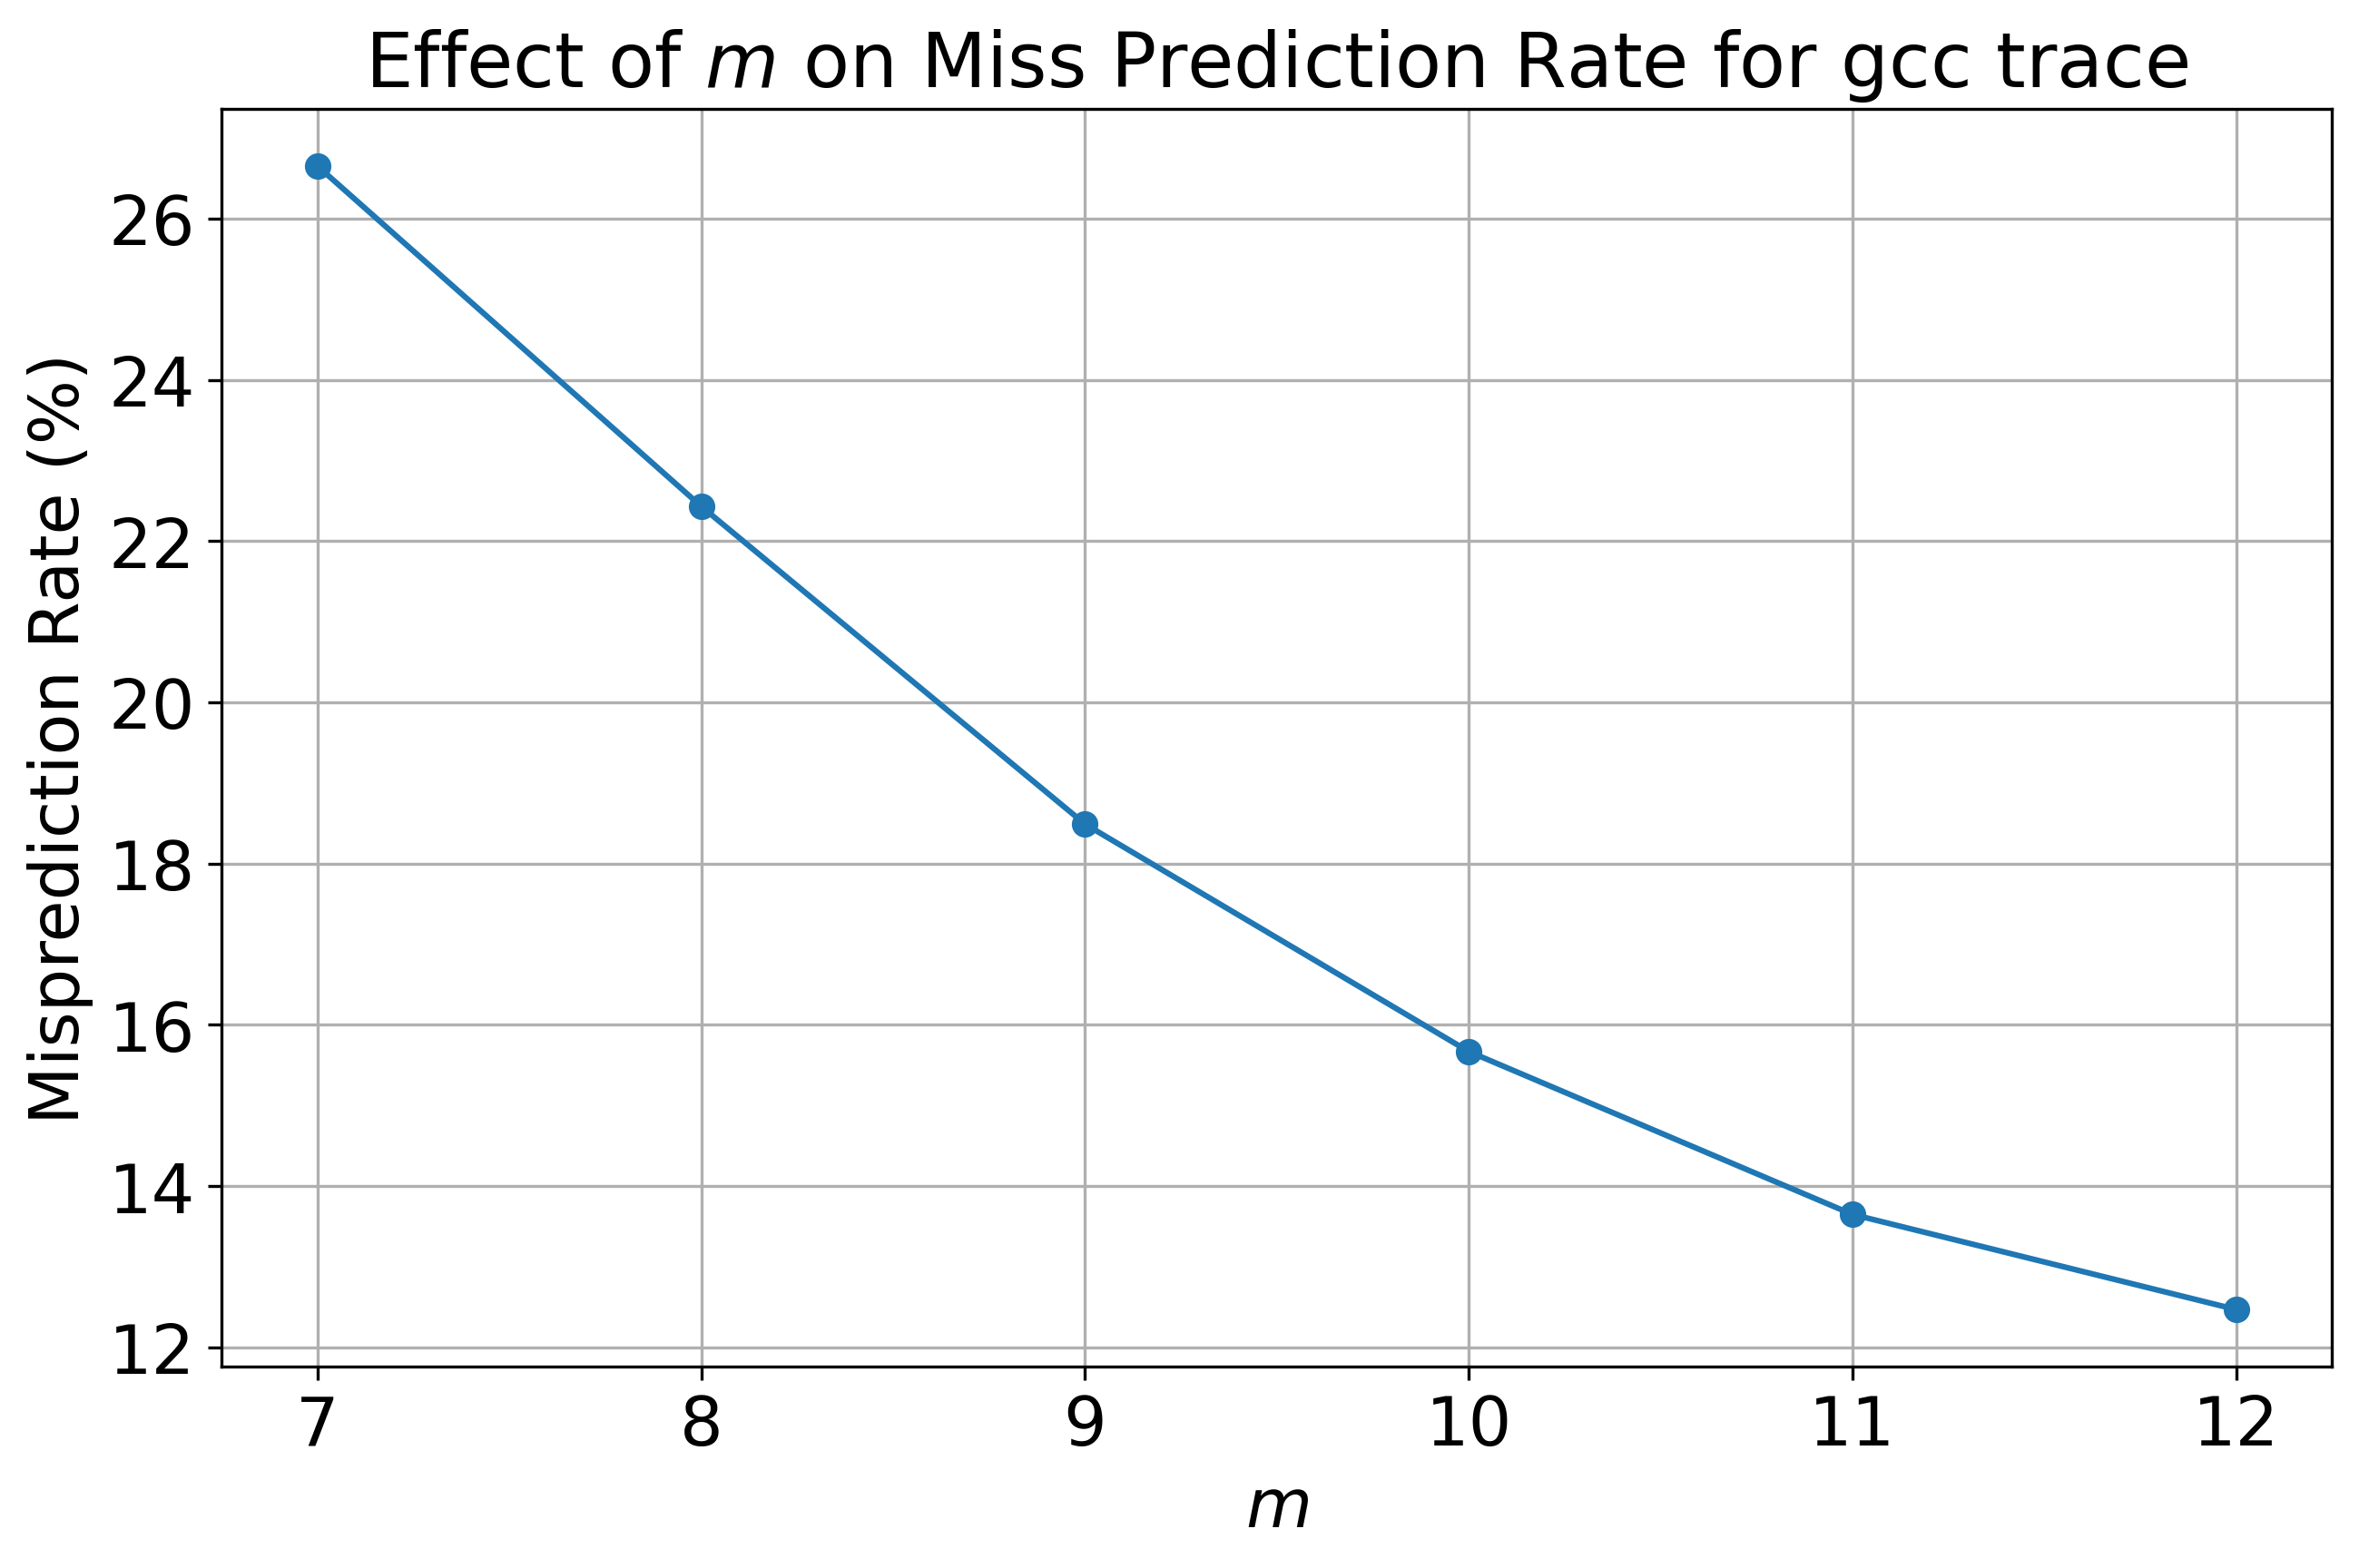
\includegraphics[width=\textwidth]{figures/fig1/fig1a1.png} % Replace with your first image
                \label{fig:pic1}
            \end{subfigure}
            \hfill
            \begin{subfigure}[b]{0.45\textwidth}
                \centering
                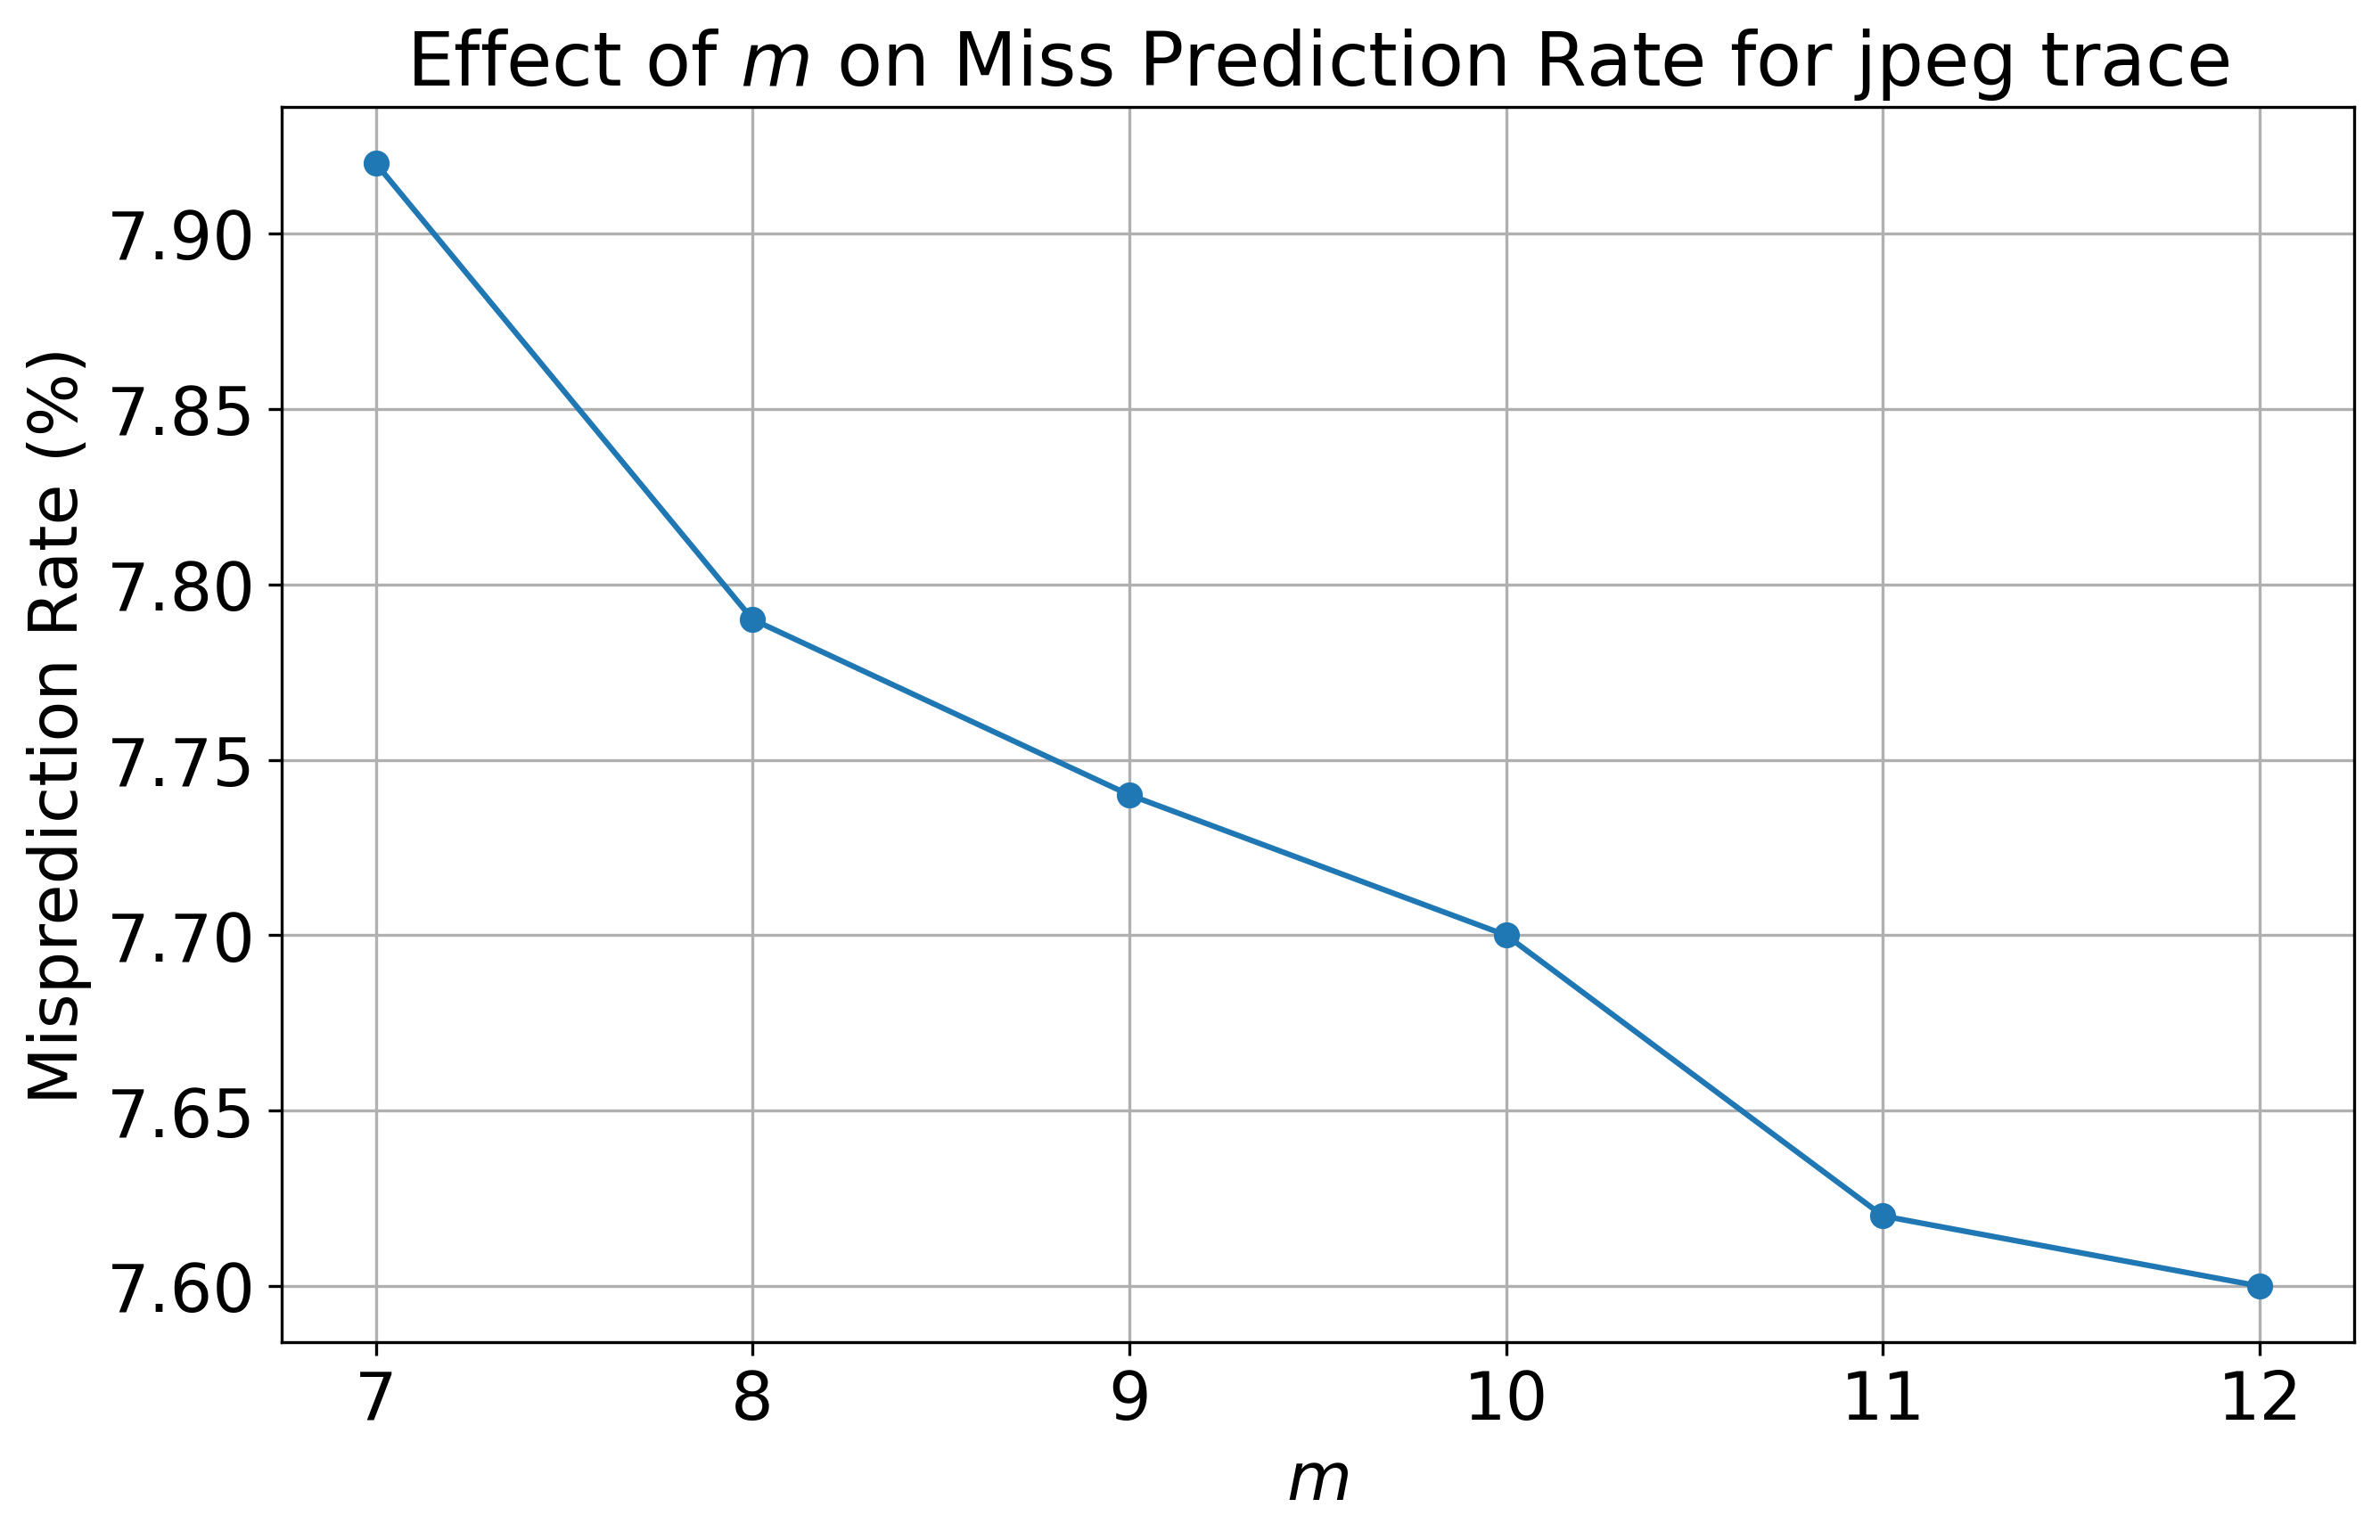
\includegraphics[width=\textwidth]{figures/fig1/fig1a2.png} % Replace with your second image
                \label{fig:pic2}
            \end{subfigure}
            \caption{Miss prediction rate for varying number of prediction bits $m$}
            \label{fig:twopictures}
        \end{figure}

        Some general observations and similarities between the plots is explained below:
        \begin{itemize}
            \item Clearly the misprediction rate decreases as we increase the number of bits $m$ used for prediction. With lesser $m$, there are collisions that happen among different branches having identical last $m+2$ bits. This mixes and garbles up the counters, leading to higher mispredictions. Having more number of bits decreases the number of collisions and thus, the misprediction rate.
            \item Clearly, there is a case of diminishing returns for both the graphs. In the left figure, we see that initially, increasing $m$ by 2 decreases the miss prediction rate by 4\%. However, at higher $m$, the same increase causes a decrease of less than 2\% for miss prediction rate. Similarly, miss prediction decrease falls from 0.1\% initially to about 0.02\% at higher $m$.   % Maybe you can add the intuitive explanation for this here
        \end{itemize}

        Some differences between the two plots are:
        \begin{itemize}
            \item Firstly, it is noteworthy that the \texttt{gcc} trace has misprediction rate in the range of 10-30\%, while the \texttt{jpeg} trace, has only 7-8\% mispredictions. This means that the \texttt{gcc} trace inherently has more \textit{unpredictable} branches compared to \texttt{jpeg} for the same number of prediction bits used for bimodal predictor. 
            \item Secondly, the fractional decrease in the misprediction rate, by increasing $m$, is much higher in \texttt{gcc} (around ~15\%) than in \texttt{jpeg} (~5-6\%). This proves that despite having more unpredictable branches than \texttt{jpeg}, the improvement in misprediction rate with increasing $m$ is much more for \texttt{gcc}. 
        \end{itemize}


        \begin{center}
            (b)
        \end{center}
    \end{subsection}

    \begin{subsection}{Gshare Predictor}
        The figure below shows the misprediction rates of the Gshare branch predictor for different values of $m$ (lookup bits from the program counter address) and $n$ (global branch history register).


        \begin{figure}[h] % Positioning option: h (here)
            \centering
            \begin{subfigure}[b]{0.45\textwidth}
                \centering
                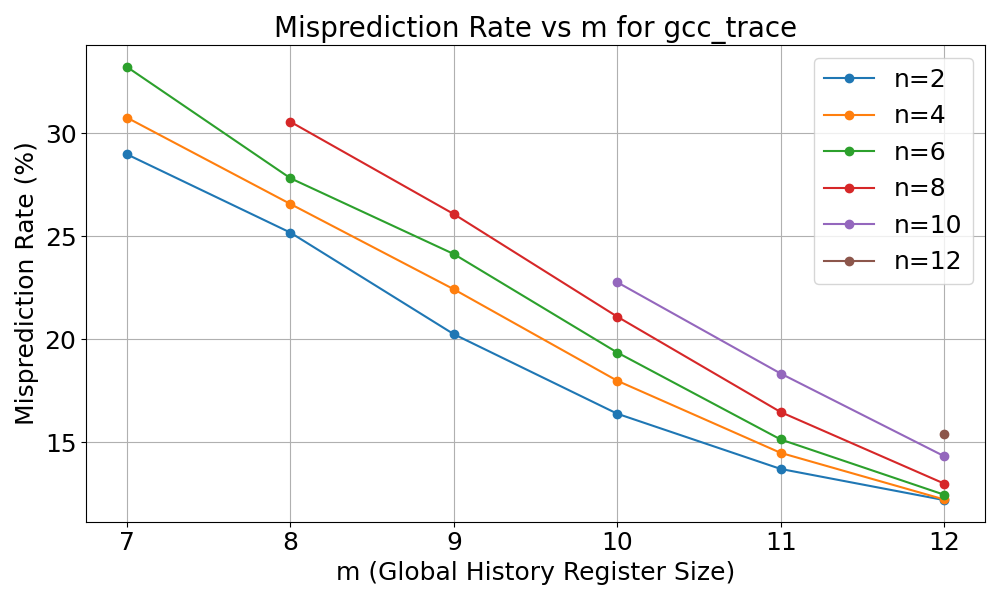
\includegraphics[width=\textwidth]{figures/fig2/gcc_misprediction_plot.png} % Replace with your first image
                \label{fig:pic1}
            \end{subfigure}
            \hfill
            \begin{subfigure}[b]{0.45\textwidth}
                \centering
                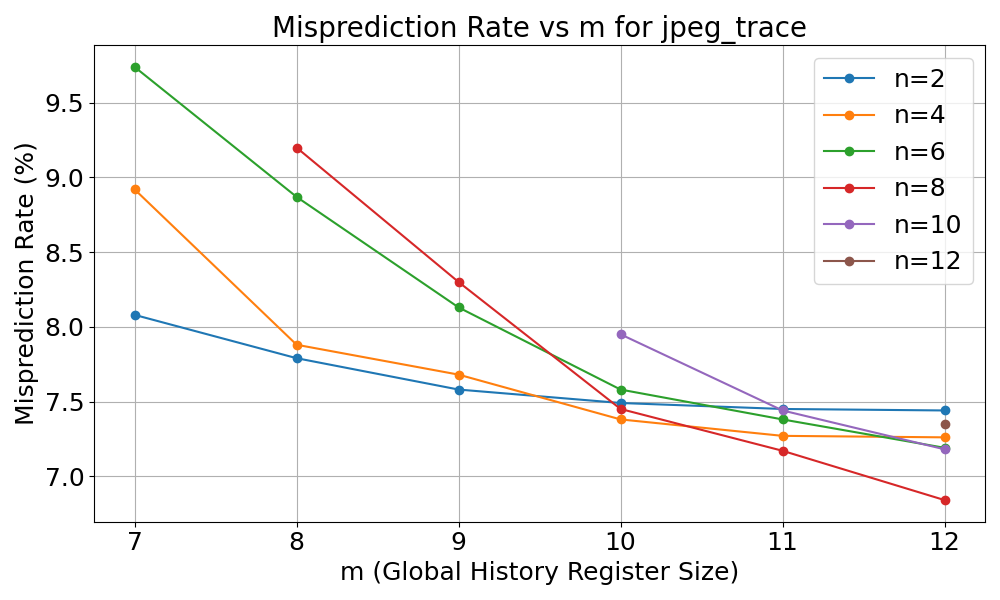
\includegraphics[width=\textwidth]{figures/fig2/jpeg_misprediction_plot.png} % Replace with your second image
                \label{fig:pic2}
            \end{subfigure}
            \caption{Miss prediction rate for varying number of prediction bits $m$ and global branch register size $n$}
            \label{fig:twopictures}
        \end{figure}

    \end{subsection}

\end{section}